\section{Neuronas Recurrentes}

Una neurona recurrente es similar a la neurona básica, a diferencia de que posee un feedback loop entre sus conexiones de salida.  En cada instante temporal, la neurona recibe una entrada y la salida del paso anterior. En el paso incial, como no hay paso incial, esta entrada es igualda a cero. 

\begin{figure}[h]
	\centering
	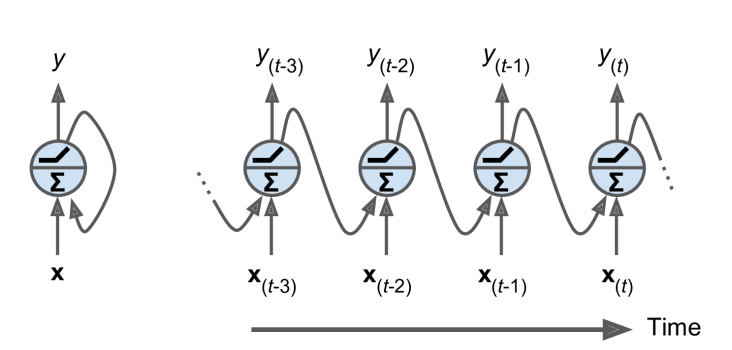
\includegraphics[scale=0.5]{images/neurona_recurrente.png}
	\caption{Neurona Recurrentey funcionamiento en tiempo}
	\label{fig:neurona}
\end{figure}

Cada neurona recurrente tiene dos conjuntos de pesos: los pesos de las entradas $w_{x}$ y los pesos de las entradas que son salidas anteriores $w_y$. Cuando se ponen varias neuronas recurrentes formando una capa, la entrada ingresa a la vez en todas las neuronas, y entre todas conforman una salida. 

\begin{figure}[h]
	\centering
	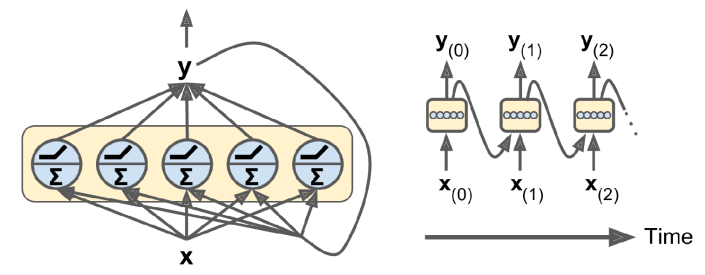
\includegraphics[scale=0.5]{images/capa_recurrente.png}
	\caption{Capa Recurrente y funcionamiento en tiempo}
	\label{fig:capa}
\end{figure}

Si se agrupan todos los pesos en matrices $W_{x}$ y $W_{y}$, la salida de la capa puede calcularse como: 

\begin{equation}
	y_{(t)} = \phi (W_x^{T} x_{(t)} + W_y^{T} y_{(t-1)} + b)
\end{equation}

Donde $\phi$ es la función de activación y $b$ es el término de bias. De esta ecuación se  puede notar que $y_{(t)}$ depende de $x_{(t)}$ y de $y_{(t-1)}$, que a su vez depende de $x_{(t-1)}$ y $y_{(t-2)}$ que a su vez es función de $x_{(t-2)}$ y  de $y_{(t-3)}$... y asi sucesivamente. Cuando una neurona es capaz de mantener un grado de información en el tiempo se habla de una \textit{memory cell} o unidad de memoria. Una neurona recurrente simple solo puede mantener información por un período corto de pasos (se considera que 10 pasos) y por eso se crean variantes que puedan manejar mayor capacidad de memoria. 

Al estado de la neurona se lo denomina $h(t)$ por \textit{hidden} y depende de las entradas y del estado anterior. La salida de la neurona también depende del estado anterior y de las entradas. En los modelos simples, el estado de la neurona y la salida pueden coincidir (como en el ejemplo anterior) pero esto puede no ser asi. En ese caso, lo que sale de la neurona y lo que se re-inyecta en la entrada no es igual. 

\begin{figure}[h]
	\centering
	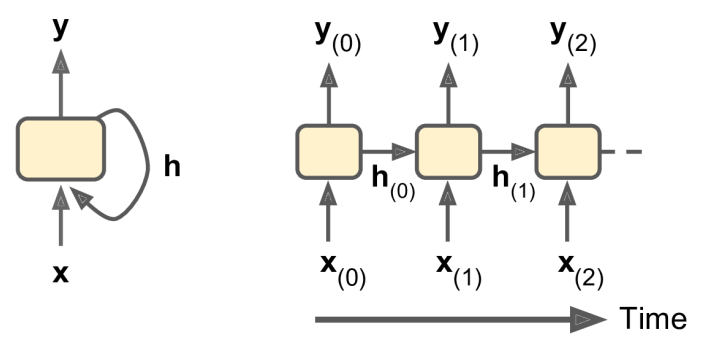
\includegraphics[scale=0.5]{images/estado.png}
	\caption{Estado oculto y salida}
	\label{fig:capa}
\end{figure}

\section{Secuencias de entrada y salida}
Las redes recurrentes se pueden configurar de acuerdo a como sean las secuencias de entrada y salida. 

\begin{itemize}
\item \textbf{Secuencia-a-Secuencia}: Simultáneamente se toma una secuencia de entradas y se genera una secuencia de salida. Es útil para predecir series temporales. 

\item \textbf{Secuencia-a-Vector}: Se toma una secuencia de entrada y se ignoran todas las salidas menos la última. Por ejemplo, la secuencia de entrada puede ser la critica de una película y la salida puede ser un puntaje de valor que exprese si esta buena o no. 

\item \textbf{Vector-a-Secuencia}: Se ingresa solo una entrada para que genere una secuencia de salida. Por ejemplo se usa en redes que reciben una imagen de entrada y generan una secuencia que la describe a la salida. 

\item \textbf{Encoder-Decoder}: Se compone de dos partes, primero una red secuencia-a-vector y despues una vector-a-secuencia. Por ejemplo se puede usar para traducir una secuencia de un lenguaje a otro. 
\end{itemize}

\section{Entrenamiento}

\subsection{Trend y Seasonality}
En muchos modelos de estimación de series temporales es estrictamente necesario quitar las tendencias y los efectos de las temporadas de la serie de datos. Por ejemplo, si se estudia el número de usuarios activos en una página, y ese número crece un 10 \% mes a mes, se debe quitar esa tendencia de los datos antes de evaluarlos. Otro ejemplo seria evaluar la venta de protector solar, donde vamos a ver una suba en las ventas en cada verano. Para quitar eso se podria calcular en lugar de la venta en un dia, la venta de un dia menos la misma venta un año atras. En los modelos de RNN no es estrictamente necesario remover estas tendencias, pero podrian llevar a un mejor resultado ya que le ahorramos al modelo tener que aprender esos patrones. 

*NOTA: Si bien en modelos de secuencia-a-secuencia puede haber mucha redundancia entre entrada y salida, por lo general el desfasaje temporal hace que la causalidad del sistema no pueda aprovechar esta redundancia. En otras palabras, al ser un sistema causal, la red solo puede ver la información del tiempo pasado y no puede aprovechar la informacion del futuro que puede estar presente en el vector objetivo. 

